\begin{name}
	{NGUYÊN HÀM - TÍCH PHÂN}
	{KT ỨNG DỤNG NGUYÊN HÀM - TÍCH PHÂN}
	{\tentruong}
	{\thoigian}
\end{name}
\setcounter{ex}{0}\setcounter{bt}{0}
\Opensolutionfile{ans}[ans/ans-2-B13-2]
\caulc
%cau1
\begin{ex}%[2D4N3-1]
	Cho hàm số $y=f(x)$ và $y=g(x)$ liên tục trên đoạn $[a;b]$. Diện tích $S$ của hình phẳng giới hạn bởi đồ thị hai hàm số $y=f(x)$, $y=g(x)$ và các đường thẳng $x=a$, $x=b$ được tính bởi công thức	
	\choice
	{\True $\displaystyle S=\int\limits_a^b |f(x)-g(x)| \mathrm dx$}
	{$\displaystyle S= \left|\int\limits_a^b [f(x)-g(x)]\mathrm dx\right|$}
	{$\displaystyle S=\int\limits_a^b |f(x)+g(x)|\mathrm dx$}
	{$\displaystyle S=\int\limits_a^b |f(x)|\mathrm dx+\int\limits_a^b |g(x)|\mathrm dx$}
	\loigiai{
	Theo định nghĩa sách giáo khoa ta có $\displaystyle S=\int\limits_a^b |f(x)-g(x)|\mathrm dx$.	
	}	
\end{ex}
%cau2
\begin{ex}%[2D4N3-3]
	Cho hàm số $ f(x)$ liên tục trên đoạn $ \left[a;b\right]$. Gọi $ (H)$ là hình phẳng giới hạn bởi đồ thị hàm số $ y=f(x)$, trục hoành và hai đường thẳng $ x=a$, $x=b$; $ V$ là thể tích của khối tròn xoay tạo đuợc khi quay $ (H)$ quanh trục $ Ox$. Khẳng định nào sau đây đúng?
	\choice
	{$ V=\pi \displaystyle\int\limits_{a}^{b} \left|f(x)\right|\mathrm{\,d}x$}
	{$ V=\displaystyle\int\limits_{a}^{b}f^2(x)\mathrm{\,d}x$}
	{\True $ V=\pi \displaystyle\int\limits_{a}^{b}f^2(x)\mathrm{\,d}x$}
	{$ V=\displaystyle\int\limits_{a}^{b}\left|f(x)\right|\mathrm{\,d}x$}
	\loigiai{
	Áp dụng công thức ta có $ V=\pi \displaystyle\int\limits_{a}^{b}f^2(x)\mathrm{\,d}x$.
	}
\end{ex} 
%cau3
\begin{ex}%[2D4N3-3]
	Thể tích khối tròn xoay tạo được do hình phẳng giới hạn bởi các đường $ y=\dfrac{x}{4}$; $y=0$; $x=1$; $x=4 $ quay quanh trục $ Ox $ là
	\choice
	{\True $ \dfrac{21\pi}{16} $}
	{$ \dfrac{15}{16} $}
	{$ \dfrac{21}{16} $}
	{$ \dfrac{15\pi}{8} $}
	\loigiai{
	Thể tích của khối tròn xoay là $\displaystyle V=\pi\int\limits_1^4\left(\dfrac{x}{4}\right)^2\mathrm{\, d}x=\left.\dfrac{\pi x^3}{48}\right|_1^4=\dfrac{21\pi}{16}$.
	}
\end{ex}
%cau4
\begin{ex}%[2D4H3-1]
	Tính diện tích $S$ của hình phẳng giới hạn bởi các đường $y = x^2 - x$ và $y = x + 3$.
	\choice
	{\True $S = \dfrac{32}{3}$}
	{$S = \dfrac{16}{3}$}
	{$S = 16$}
	{$S = 32$}
	\loigiai{Xét phương trình hoành độ giao điểm \begin{align*}
	x^2 - 2x - 3 = 0 \Leftrightarrow \hoac{& x = -1 \\ & x = 3.}
	\end{align*}
	Diện tích $S$ cần tìm là
	$S = \displaystyle \int\limits_{-1}^3 \left| x^2 - 2x - 3 \right|\mathrm{\, d}x = \dfrac{32}{3}$.
	}
\end{ex}
%cau5
\begin{ex}%[2D4N3-4]
	Viết công thức tính thể tích $V$ của vật thể nằm giữa hai mặt phẳng $x=0$ và $x=\ln 4$, biết khi cắt vật thể bởi mặt phẳng vuông góc với trục hoành tại điểm có hoành độ $x$ ($0\le x\le \ln 4$), ta được thiết diện là một hình vuông có độ dài cạnh là $\sqrt{x\mathrm{e}^x}$.
	\choice
	{\True $V=\displaystyle\int\limits_0^{\ln 4}x\mathrm{e}^x\mathrm{\,d}x$}
	{$V=\pi\displaystyle\int\limits_0^{\ln 4}x\mathrm{e}^x\mathrm{\,d}x$}
	{$V=\pi\displaystyle\int\limits_0^{\ln 4}\left(x\mathrm{e}^x\right)^2\mathrm{\,d}x$}
	{$V=\displaystyle\int\limits_0^{\ln 4}\sqrt{x\mathrm{e}^x}\mathrm{\,d}x$}
	\loigiai{
	Theo định nghĩa ta có $V=\displaystyle\int\limits_0^{\ln 4}x\mathrm{e}^x\mathrm{\,d}x$.
	}
\end{ex}
%cau6
\begin{ex}%[2D4H3-4]
	Tính thể tích $V$ của phần vật thể giới hạn bởi hai mặt phẳng $x=0$ và $x=3$, biết rằng thiết diện của vật thể bị cắt bởi mặt phẳng vuông góc với trục $Ox$ tại điểm có hoành độ $x$ ($0\leq x \leq 3$) là một hình tròn có đường kính bằng $\sqrt{36-3x^2}$.
	\choice
	{\True $V=\dfrac{81\pi}{4}$}
	{$V=\dfrac{81}{4}$}
	{$V=81\pi$}
	{$V=81$}
	\loigiai
	{
	Diện tích của thiết diện đó là $S(x)=\pi\cdot \left(\dfrac{\sqrt{36-3x^2}}{2}\right)^2 = \dfrac{\pi}{4}\cdot(36-3x^2)$.\\
	Thể tích vật thể tròn xoay đó là
	\begin{eqnarray*}
	V=\displaystyle\int\limits_0^3\dfrac{\pi}{4}\cdot(36-3x^2)\mathrm{\,d}x = \dfrac{\pi}{4} \displaystyle\int\limits_0^3(36-3x^2)\mathrm{\,d}x = \dfrac{\pi}{4}\cdot(36x-x^3)\bigg|_0^3 = \dfrac{81\pi}{4}.
	\end{eqnarray*}
	}
\end{ex}
%cau7
\begin{ex}%[2D4H3-1]
	Hình phẳng giới hạn bởi các đường $y=x^3+1$, $y=0$, $x=0$, $x=1$ có diện tích bằng
	\choice
	{\True $\dfrac{5}{4}$}
	{$\dfrac{7}{4}$}
	{$\dfrac{4}{3}$}
	{$\dfrac{3}{4}$}
	\loigiai{
	Diện tích hình phẳng giới hạn bởi các đường $y=x^3+1$, $y=0$, $x=0$, $x=1$ là
	$$S=\displaystyle\int\limits_0^1\left|x^3+1\right|\mathrm{\,d}x=\displaystyle\int\limits_0^1\left(x^3+1\right)\mathrm{\,d}x =\left.\left(\dfrac{x^4}{4}+x\right)\right|_0^1=\dfrac{5}{4}.$$
	}
\end{ex}
%cau8
\begin{ex}%[2D4H3-1]
	\immini
	{Gọi tam giác cong $(OAB)$ là hình phẳng giới hạn bởi đồ thị các hàm số $y=2x^2$, $y=3-x$, $y=0$ (hình vẽ bên). Tính diện tích $S$ của $(OAB)$.
	\choice
	{\True $S=\dfrac{8}{3}$}
	{$S=\dfrac{4}{3}$}
	{$S=\dfrac{5}{3}$}
	{$S=\dfrac{10}{3}$}
	}
	{\begin{tikzpicture}[>=stealth,x=1cm,y=1cm,scale=0.55]
	\draw[->] (-2.2,0)--(4.5,0) node[below]{$x$};
	\draw[->] (0,-1) --(0,5.2) node[right]{$y$};
	\draw [samples=100, domain=-1.6:1.6] plot (\x, {2*(\x)^2});
	\draw [samples=100, domain=-2.2:4] plot (\x, {3-(\x)});
	\fill [pattern=north west lines,draw=none] (0,0)-- plot[domain=0:1] (\x, {2*(\x)^2})-- plot[domain=1:3] (\x, {3-\x})--(0,0);
	\fill (0,0) node[shift={(-120:1.5ex)}]{\footnotesize$O$} circle(1pt);
	\fill (3,0) node[shift={(-90:1.5ex)}]{\footnotesize$3$} circle(1pt);
	\fill (1,0) node[shift={(-90:1.5ex)}]{\footnotesize$1$} circle(1pt);
	\fill (0,3) node[shift={(0:1.5ex)}]{\footnotesize$3$} circle(1pt);
	\draw (3,0) node[shift={(90:1.5ex)}]{\footnotesize$B$};
	\fill (1,2) node[shift={(0:1.5ex)}]{\footnotesize $A$} circle(1pt);
	\end{tikzpicture}}
	\loigiai
	{
	\immini
	{
	Xét phương trình hoành độ giao điểm
	\[2x^2=3-x\Leftrightarrow2x^2+x-3=0\Leftrightarrow\hoac{&x=1\\&x=-\dfrac{3}{2}.}\]
	Ta có 
	\begin{eqnarray*}
	S_{OAB}&=&\displaystyle\int\limits_0^1 2x^2\mathrm{\,d}x+\displaystyle\int\limits_1^3 (3-x)\mathrm{\,d}x
	=\dfrac{2}{3}x^3\bigg|_0^1+\left(3x-\dfrac{x^2}{2}\right)\bigg|_1^3=\dfrac{8}{3}.
	\end{eqnarray*}
	}
	{\begin{tikzpicture}[>=stealth,x=1cm,y=1cm,scale=0.55]
	\draw[->] (-2.2,0)--(4.5,0) node[below]{$x$};
	\draw[->] (0,-1) --(0,5.2) node[right]{$y$};
	\draw [samples=100, domain=-1.6:1.6] plot (\x, {2*(\x)^2});
	\draw [samples=100, domain=-2.2:4] plot (\x, {3-(\x)});
	\fill [pattern=north west lines,draw=none] (0,0)-- plot[domain=0:1] (\x, {2*(\x)^2})-- plot[domain=1:3] (\x, {3-\x})--(0,0);
	\fill (0,0) node[shift={(-120:1.5ex)}]{\footnotesize$O$} circle(1pt);
	\fill (3,0) node[shift={(-90:1.5ex)}]{\footnotesize$3$} circle(1pt);
	\fill (1,0) node[shift={(-90:1.5ex)}]{\footnotesize$1$} circle(1pt);
	\fill (0,3) node[shift={(0:1.5ex)}]{\footnotesize$3$} circle(1pt);
	\draw (3,0) node[shift={(90:1.5ex)}]{\footnotesize$B$};
	\fill (1,2) node[shift={(0:1.5ex)}]{\footnotesize $A$} circle(1pt);
	\draw[dashed] (1,2)--(1,0);
	\end{tikzpicture}}
	}
\end{ex}
%cau9
\begin{ex}%[2D4H3-1]
	Diện tích hình phẳng giới hạn bởi hai đồ thị hàm số $ y = x^3 - 12x $ và $ y = x^2 $ là
	\choice
	{$ S = \dfrac{939}{12} $}
	{$ S = \dfrac{979}{12} $}
	{$ S = \dfrac{160}{3} $}
	{\True $ S = \dfrac{937}{12} $}
	\loigiai{
	Hoành độ giao điểm của hai đồ thị hàm số là nghiệm của phương trình 
	$$ x^3-12x=x^2\Leftrightarrow \hoac{&x=-3 \\& x=0 \\& x=4.}$$
	Diện tích hình phẳng cần tìm là
	\[ 
	S=\int\limits_{-3}^0 (x^3-12x-x^2) \mathrm{\,d}x+\int\limits_{0}^{4} (x^2-x^3+12x) \mathrm{\,d}x=\dfrac{937}{12}.
	\]
	}
\end{ex}
%cau10
\begin{ex}%[2D4H3-4]
	Cho phần vật thể $\left( \Im \right)$ giới hạn bởi hai mặt phẳng có phương trình $x = 0$ và $x = 2$. Cắt phần vật thể $\left(\Im\right)$ bởi mặt phẳng vuông góc với trục $Ox$ tại điểm có hoành độ $x$ $\left({0 \leq x \leq 2} \right)$, ta được thiết diện là một tam giác đều có độ dài cạnh bằng $x\sqrt{2 - x} $. Tính thể tích $V$ của phần vật thể $\left( \Im \right)$.
	\choice
	{$V = \dfrac{4}{3}$}
	{\True $V = \dfrac{\sqrt 3 }{3}$}
	{$V = 4\sqrt 3$}
	{$V = \sqrt 3$}
	\loigiai{
	Diện tích thiết diện: $S_\triangle = \dfrac{x^2\left({2 - x}\right)\sqrt 3}{4}$.\\
	$V_\Im = \displaystyle\int\limits_0^{2} \dfrac{x^2\left(2 - x\right)\sqrt 3 }{4}\mathrm{\,d}x =\dfrac{\sqrt 3 }{4}\displaystyle\int\limits_0^{2} x^2\left(2 - x\right)\mathrm{\,d}x= \left.{\dfrac{\sqrt 3}{4}\left(\dfrac{2}{3} x^3 - \dfrac{1}{4}x^4 \right)}\right|_0^2 = \dfrac {\sqrt 3}{3}$.}
\end{ex}
%cau11
\begin{ex}%[2D4V3-1]
	Biết diện tích hình phẳng giới hạn bởi đồ thị hàm số $y=3x^2+2mx+m^2+1$, trục hoành, trục tung và đường thẳng $x=\sqrt{2}$ đạt giá trị nhỏ nhất. Mệnh đề nào sau đây đúng?
	\choice
	{$m\in(-4;-1)$}
	{$m\in(3;5)$}
	{$m\in(0;3)$}
	{\True $m\in(-2;1)$}
	\loigiai{
	Ta có $y=(x+m)^2+2x^2+1>0,\ \forall x\in\mathbb{R}$.\\
	Diện tích hình phẳng cần tìm là
	\begin{eqnarray*}
	S &=& \int\limits_0^{\sqrt{2}} \left|3x^2+2mx+m^2+1\right|\mathrm{\,d}x \\
	&=& \int\limits_0^{\sqrt{2}} \left(3x^2+2mx+m^2+1\right)\mathrm{\,d}x \\
	&=& \left(x^3+mx^2+m^2x+x\right)\Big|_0^{\sqrt{2}} \\
	&=& \sqrt{2}m^2+2m+3\sqrt{2}\\
	&=& \sqrt{2}\left(m+\dfrac{\sqrt{2}}{2}\right)^2+\dfrac{5\sqrt{2}}{2}\ge \dfrac{5\sqrt{2}}{2}.
	\end{eqnarray*}
	Vậy $S$ đạt giá trị nhỏ nhất bằng $\dfrac{5\sqrt{2}}{2}$ khi và chỉ khi $m=-\dfrac{\sqrt{2}}{2}\approx -0{,}7071$.
	}
\end{ex}
%cau12
\begin{ex}%[2D4V3-3]
	Tính thể tích khối tròn xoay được tạo bởi phép quay quanh trục $Ox$ của hình phẳng giới hạn bởi các đường $y=\sqrt{x}$, $y=2-x$ và trục hoành.
	\choice
	{$\pi$}
	{$\dfrac{3\pi}{2}$}
	{\True $\dfrac{5\pi}{6}$}
	{$\dfrac{2\pi}{3}$}
	\loigiai{
	\immini{Xét các phương trình sau
	\begin{itemize}
	\item $\sqrt{x} = 0 \Leftrightarrow x=0$.
	\item $\sqrt{x} = 2-x \Leftrightarrow \left(\sqrt{x}\right)^2 + \sqrt{x} -2 =0 \Leftrightarrow x=1$.	
	\item $2-x=0 \Leftrightarrow x=2$.
	\end{itemize}
	Thể tích của khối tròn xoay cần tính là 
	}
	{\begin{tikzpicture}[scale=0.8, font=\footnotesize, line join = round, line cap = round, >=stealth]
	\draw[->](-1,0) -- (0,0) node[below left]{$O$} -- (4,0) node[below]{$x$};
	\draw[->](0,-1.5) -- (0,3) node[right]{$y$};
	\foreach \x in {1,2} \draw (\x,0) node[below]{$\x$} circle(1pt);	
	\draw[domain=0:3,samples=100] plot(\x,{(\x)^0.5}) node[below]{$y=\sqrt{x}$};	
	\draw[domain=-0.5:3,samples=100] plot(\x,{2-\x}) node[left]{$y=2-x$};	
	\draw[pattern = north east lines, draw=none] (0,0) plot[domain=0:1] (\x, {(\x)^0.5})--(2,0)--cycle;
	\draw[dashed] (1,1)--(1,0);
	\end{tikzpicture}
	}
	\allowdisplaybreaks
	\begin{eqnarray*}
	V &=& \pi \displaystyle \int\limits_{0}^{1} \left(\sqrt{x}\right)^2 \mathrm{\,d}x + \pi \displaystyle \int\limits_{1}^{2} (2-x)^2 \mathrm{\,d}x = \pi \displaystyle \int\limits_{0}^{1} x \mathrm{\,d}x + \pi \displaystyle \int\limits_{1}^{2} \left(4-4x+x^2\right) \mathrm{\,d}x\\	
	&=& \pi	\cdot \dfrac{x^2}{2} \bigg|_{0}^{1}	 + \pi	\cdot \left(4x - 2x^2 + \dfrac{x^3}{3}\right) \bigg|_{1}^{2} = \dfrac{\pi}{2} + \dfrac{\pi}{3} = \dfrac{5\pi}{6}.
	\end{eqnarray*}
	}	
\end{ex}
\Closesolutionfile{ans}
% \indapan{6}{ans/ans-2-B13-2}
\cauds
\Opensolutionfile{ans}[ans/ans-2-B13-2-DS]
\begin{ex}%[2D4V3-1]
	Cho hình $(H)$ giới hạn bởi các đường $y=\dfrac{2}{x}$, $y=0$, $x=1$ và $x=4$.
	\choiceTF
	{\True Số $m$ thỏa mãn $\displaystyle\int\limits_1^m\dfrac{1}{x}\mathrm{\, d}x=2$ là $\mathrm{e}^2$}
	{\True Diện tích hình $(H)$ bằng $4\ln 2$}
	{Thể tích của khối tròn xoay khi quay hình $(H)$ xung quanh trục hoành bằng $2\pi$}
	{Gọi $x=k$ là đường thẳng chia hình $(H)$ thành $2$ phần có diện tích bằng nhau. Khi đó $k=1$}
	\loigiai{
	\begin{center}
	\begin{tikzpicture}[scale=1, font=\footnotesize, line join=round, line cap=round, >=stealth]
	\draw[->] (-1,0)--(4.5,0) node[below] {$x$} ;
	\draw[->] (0,-0.6)--(0,2.5) node[right] {$y$} ;
	\draw[fill=black] (0,0) node[below left] {$O$};
	\draw[domain=0.8:4.4] plot(\x,{2/(\x)}) ;
	\draw[color=black,fill=black,pattern=north east lines,pattern color=black] {[smooth,samples=100,domain=1:4] plot(\x,{2/(\x)})} -- (4, 0)-- (1,0) -- cycle;
	\draw[dashed] (2,-.61)--(2,2) node[below right] {$x=k$};
	\draw (1,0) node[below] {$1$};
	\draw(4,0) node[below]{$4$};
	\fill (1,0) circle (1pt) (0,0) circle (1pt) (4,0) circle (1pt);
	\end{tikzpicture}
	\end{center}
	\begin{itemchoice}
	\itemch Đúng. Vì $\displaystyle\int\limits_1^m\dfrac{1}{x}\mathrm{\, d}x=2\Leftrightarrow \left(\ln x\right)\bigg|_1^m=2\Leftrightarrow \ln m=2\Leftrightarrow m=\mathrm{e}^2$.
	\itemch Đúng. Diện tích hình $(H)$ bằng $S=\displaystyle\int\limits_1^4\dfrac{2}{x}\mathrm{\, d}x=4\ln 2$.
	\itemch Sai. Thể tích của khối tròn xoay cần tính là
	$$V=\pi \displaystyle\int\limits_1^4\left(\dfrac{2}{x}\right)^2\mathrm{\,d}x=\pi \displaystyle\int\limits_1^4\dfrac{4}{x^2}\mathrm{\,d}x= 4\pi \cdot \left(-\dfrac{1}{x}\right)\bigg|_{1}^4 = 3\pi. $$
	\itemch Đường thẳng $x=k$ chia hình $(H)$ thành $2$ phần có diện tích bằng nhau nên $$\displaystyle\int\limits_1^k\dfrac{2}{x}\mathrm{\, d}x=2\ln 2\Leftrightarrow \left(2\ln x\right)\bigg|_1^k=2\ln 2\Leftrightarrow 2\ln k=2\ln 2\Leftrightarrow k=2.$$
	\end{itemchoice}
	}
\end{ex}
\begin{ex}%[2D4V3-1]
	Đồ thị của hàm số $y=f(x)$ liên tục trên đoạn $[-3;5]$ như hình vẽ dưới đây (phần cong của đồ thị là một phần của Parabol $y=ax^2+bx+c$).
	\begin{center}
	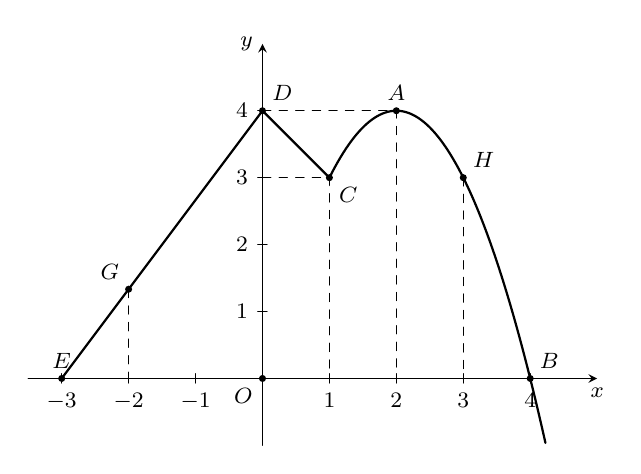
\begin{tikzpicture}[>=stealth,line join=round,line cap=round,font=\footnotesize,scale=0.85]
	\draw[->] (0,-1)--(0,5)node[left]{$y$};
	\foreach \y in {1,2,3,4} \draw[shift={(0,\y)}] (2pt,0)--(-2pt,0) node[left] {\footnotesize $\y$};
	\draw[->] (-3.5,0)--(5,0)node[below]{$x$};
	\foreach \x in {-3,-2,-1,1,2,3,4} \draw[shift={(\x,0)}] (0,2pt)--(0,-2pt) node[below] {\footnotesize $\x$};
	\draw[thick] (-3,0)--(0,4)--(1,3) plot[smooth,samples=200,domain=1:4.23] (\x,{-(\x)^2+4*\x});
	\draw[dashed] (-2,4/3)--(-2,0) (0,3)--(1,3)--(1,0) (0,4)--(2,4)--(2,0) (3,3)--(3,0);
	\fill (0,0)node[below left]{$O$}circle(1.5pt) (-3,0)node[above]{$E$}circle(1.5pt) (-2,4/3)node[above left]{$G$}circle(1.5pt) (0,4)node[above right]{$D$}circle(1.5pt) (1,3)node[below right]{$C$}circle(1.5pt) (2,4)node[above]{$A$}circle(1.5pt) (3,3)node[above right]{$H$}circle(1.5pt) (4,0)node[above right]{$B$}circle(1.5pt);
	\end{tikzpicture}
	\end{center}
	\choiceTF
	{\True Diện tích tam giác $ODE$ bằng $6$}
	{\True Diện tích hình phẳng giới hạn bởi Parabol và đường thẳng $CB$ bằng $\dfrac{9}{2}$}
	{\True Giá trị của $I=\displaystyle\int\limits_{-2}^3 f(x)\mathrm{\,d}x$ bằng $\dfrac{97}{6}$}
	{Gọi diện tích tam giác $OED$ là $S_1$ và diện tích hình phẳng giới hạn bởi phần cong Parabol, trục $Ox$ và đường thẳng $x=1$ là $S_2$. Khi đó $3S_1>2S_2$}
	\loigiai{
	\begin{itemize}
	\item Đường thẳng đi qua $E$, $D$ là $y=\dfrac{4}{3}x+4$.
	\item Đường thẳng đi qua $B$, $C$ là $y=-x+4$.
	\item Đường thẳng đi qua $D$, $C$ là $y=-x+4$.
	\item Parabol có phương trình là $y=-x^2+4x$.
	\end{itemize}
	Do đó $y=f(x)=\heva{&\dfrac{4}{3}x+4&\textrm{ nếu }-3\le x< 0\\ &-x+4&\textrm{ nếu }0\le x<1\\ &-x^2+4x&\textrm{ nếu }1\le x\le 5.}$ 
	\begin{itemchoice}
	\itemch Đúng. Diện tích tam giác $ODE$ bằng $\displaystyle\int\limits_{-3}^{0}\left(\dfrac{4}{3}x+4\right)\mathrm{\, d}x=6$.
	\itemch Đúng. Diện tích hình phẳng giới hạn bởi Parabol và đường thẳng $CB$ bằng
	$$\displaystyle\int\limits_1^3\left((-x^2+4x)-(-x+4)\right)\mathrm{\, d}x=\displaystyle\int\limits_1^3\left(-x^2+5x-4\right)\mathrm{\, d}x=\dfrac{9}{2}.$$
	\itemch Đúng. Ta có
	{\allowdisplaybreaks
	\begin{align*}
	I&=\displaystyle\int\limits_{-2}^3 f(x)\mathrm{\,d}x\\
	&=\displaystyle\int\limits_{-2}^0 f(x)\mathrm{\,d}x+\displaystyle\int\limits_0^1 f(x)\mathrm{\,d}x+\displaystyle\int\limits_1^3 f(x)\mathrm{\,d}x\\
	&=\displaystyle\int\limits_{-2}^0 \left(\dfrac{4}{3}x+4\right)\mathrm{\,d}x+\displaystyle\int\limits_0^1 (-x+4)\mathrm{\,d}x+\displaystyle\int\limits_1^3 (-x^2+4x)\mathrm{\,d}x\\
	&=\left.\left(-\dfrac{2x^2}{3}+4x\right)\right|_{-2}^0+\left.\left(-\dfrac{x^2}{2}+4x\right)\right|_0^1+\left.\left(-\dfrac{x^3}{3}+2x^2\right)\right|_1^3\\
	&=\dfrac{97}{6}.
	\end{align*}}
	\itemch Sai. Diện tích tam giác $OED$ là $S_1=6$ và diện tích hình phẳng giới hạn bởi phần cong Parabol, trục $Ox$ và đường thẳng $x=1$ là $S_2=\displaystyle\int\limits_1^4(-x^2+4x)\mathrm{\, d}x=9$. Do đó $3S_1=2S_2$.
	\end{itemchoice}
	}
\end{ex}
\begin{ex}%[2D4V3-1]
\immini{
	Cho hàm số $y=x^4-x^2+m$ có đồ thị là $(C)$ cắt trục hoành tại $4$ điểm phân biệt. Gọi $S_1$ là diện tích hình phẳng giới hạn bởi trục hoành và đồ thị $(C)$ nằm phía trên trục hoành, $S_2$ là diện tích hình phẳng giới hạn bởi trục hoành và phần đồ thị $(C)$ nằm phía dưới trục hoành, $S$ là diện tích hình phẳng giới hạn bởi trục hoành và đồ thị $(C)$.
}{
	\begin{tikzpicture}[scale=0.85,thick,>=stealth,x=0.9cm,
	y=0.9cm]
	\draw[thin,->](-2.2,0)--(2.0,0) node[below]{$x$};
	\draw[thin,->](0,-1.1)--(0,2.0) node[left]{$y$};
	\node[below left](0,0){$O$};
	\draw[smooth,samples=100,domain=-1.8:1.8]
	plot(\x,{(\x)^4-3*(\x)^2+5/4});
	\fill[pattern=north west lines, domain=-0.71:0.71] plot (\x, {(\x)^4-3*(\x)^2+5/4})-- (-0.71,0) -- (0.71,0) -- cycle;
	\fill[pattern=dots, domain=-1.58:-0.71] plot (\x, {(\x)^4-3*(\x)^2+5/4})-- (-0.71,0) -- (-1.58,0) -- cycle;
	\fill[pattern=dots, domain=0.71:1.58] plot (\x, {(\x)^4-3*(\x)^2+5/4})-- (1.58,0) -- (0.71,0) -- cycle;
	\end{tikzpicture}
}
	\choiceTF
	{Khi $m=1$ thì diện tích $S=1$}
	{\True Khi $m=-2$ thì diện tích $S=\dfrac{56}{15}\sqrt{2}$}
	{Khi $m=0$ thì diện tích $S=\dfrac{1}{4}$}
	{\True Biết rằng $S_1=S_2$ và giá trị của $m=\dfrac{a}{b}$ với $\dfrac{a}{b}$ là phân số tối giản. Khi đó $T=a^2+b^2=1321$}
	\loigiai{
	\begin{itemchoice}
	\itemch Sai. Khi $m=1$, xét phương trình $x^4-x^2+1=0$. Phương trình vô nghiệm nên diện tích $S=0$.
	\itemch Đúng. Khi $m=-2$, xét phương trình $x^4-x^2-2=0\Leftrightarrow \hoac{&x=\sqrt{2}\\&x=-\sqrt{2}}$. Khi đó $$S=\displaystyle\int\limits_{-\sqrt{2}}^{\sqrt{2}}\left|x^4-x^2-2\right|\mathrm{\, d}x=\dfrac{56}{15}\sqrt{2}.$$
	\itemch Sai. Khi $m=0$, xét phương trình $x^4-x^2=0\Leftrightarrow\hoac{&x=-1\\&x=0\\&x=1}$. Khi đó $$S=\displaystyle\int\limits_{-1}^{1}\left|x^4-x^2\right|\mathrm{\, d}x=\dfrac{4}{15}.$$
	\itemch \immini
	{Phương trình hoành độ giao điểm của $(C)$ và trục hoành: $x^4-x^2+m=0\quad (1)$. Đặt $t=x^2$, $t\geq 0$, ta được phương trình $t^2-t+m=0\quad (2)$.\\ Ta có $(C)$ cắt trục hoành tại bốn điểm phân biệt $\Leftrightarrow$ $(2)$ có hai nghiệm cùng dương $$\Leftrightarrow\heva{&\Delta>0\\&S>0\\&P>0}\Leftrightarrow\heva{&1-4m>0\\&3>0\\&m>0}\Leftrightarrow 0<m<\dfrac{1}{4}.$$
	}
	{
	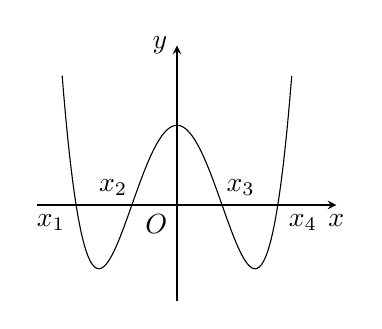
\begin{tikzpicture}[scale=0.9,>=stealth,x=0.9cm,
	y=0.9cm]
	\draw[->](-2.2,0)--(2.5,0) node[below]{$x$};
	\draw[->](0,-1.5)--(0,2.5) node[left]{$y$};
	\draw (-1,0)node[above]{$x_2$} (1,0)node[above]{$x_3$}
	(-1.6,0)node[below left]{$x_1$}
	(1.6,0)node[below right]{$x_4$};
	\node[below left](0,0){$O$};
	\draw[smooth,samples=100,domain=-1.8:1.8] plot(\x,{(\x)^4-3*(\x)^2+5/4});
	\end{tikzpicture}
	}
	\noindent	Gọi các nghiệm của phương trình $(1)$ là $x_1<x_2<x_3<x_4$, $x_1,\ x_2,\ x_3,\ x_4\neq 0$. Do đồ thị $(C)$ nhận trục tung là trục đối xứng nên ta có yêu cầu bài toán thỏa mãn khi và chỉ khi
	$$\displaystyle\int\limits_{0}^{x_4}(x^4-3x^2+m)\mathrm{\, d}x =0 \Leftrightarrow 3x_4^4-5x_4^2+15m=0.$$
	Mặt khác $x_4$ là nghiệm của phương trình (1) nên ta có 
	$$x_4^4-x_4^2+m=0.$$
	Do đó ta có 
	$$\heva{&x_4^4-x_4^2+m=0\\&3x_4^3-5x_4^2+15m=0 } \Leftrightarrow \heva{& x_4^2=\dfrac{5}{6}\\&m=\dfrac{5}{36}.}$$
	Ta thấy $m=\dfrac{5}{36}$ thỏa yêu cầu bài toán. \\
	Vậy $ T=5^2+36^2=1321.$
	\end{itemchoice}
	}
\end{ex}
\begin{ex}%[2D4V3-3]
	Cho đồ thị $(C)\colon y=f(x)=\sqrt{x}$. Gọi $(H)$ là hình phẳng giới hạn bởi $(C)$, đường thẳng $x=9$, trục hoành. Cho $M$ là điểm thuộc $(C)$, $A(9;0)$. Gọi $V_1$ là thể tích khối tròn xoay khi cho $(H)$ quay quanh trục $Ox$, $V_2$ là thể tích khối tròn xoay khi cho tam giác $AOM$ quay quanh trục $Ox$.
	\begin{center}
	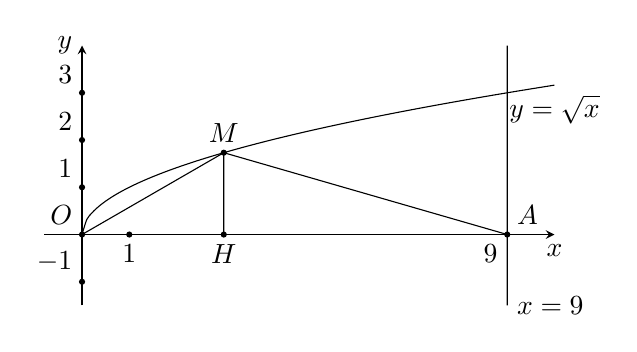
\begin{tikzpicture}[scale=0.6,>=stealth]
	\draw[->](-0.8,0)--(10,0)node[below]{$x$};
	\draw[->](0,-1.5)--(0,4)node[left]{$y$};
	\draw[smooth,samples=100,domain=0:10]plot(\x,{sqrt(\x)})node[below]{$y=\sqrt{x}$};
	\draw(0,0)node[above left]{$O$}--(3,{sqrt(3)})node[above]{$M$}--(9,0)node[above right]{$A$} (3,{sqrt(3)})--(3,0) (9,4)--(9,-1.5)node[right]{$x=9$};
	\draw[fill](0,-1)node[above left]{$-1$}circle(1.5pt) (0,1)node[above left]{$1$}circle(1.5pt) (0,2)node[above left]{$2$}circle(1.5pt) (0,3)node[above left]{$3$}circle(1.5pt) (1,0)node[below]{$1$}circle(1.5pt) (3,0)node[below]{$H$}circle(1.5pt) (9,0)node[below left]{$9$}circle(1.5pt) (0,0)circle(1.5pt) (3,{sqrt(3)})circle(1.5pt);
	\end{tikzpicture}
	\end{center}
	\choiceTF
	{Diện tích hình phẳng giới hạn bởi đồ thị $(C)$, đường thẳng $x=9$ và trục $Oy$ bằng $S_1=16$}
	{\True $V_1=\dfrac{81}{2}\pi$}
	{Gọi $N(4;2)$ thuộc $(C)$. Khi đó thể tích khối tròn xoay khi quay tam giác $AON$ quay xung quanh trục $Ox$ là $V=11\pi$}
	{\True Diện tích $S$ phần hình phẳng giới hạn bởi $(C)$ và $OM$ biết $V_1=2V_2$ là $S=\dfrac{27\sqrt{3}}{16}$}
	\loigiai{
	\begin{itemchoice}
	\itemch Sai. Ta có $S_1=\displaystyle\int\limits_0^9\sqrt{x}\mathrm{\, d}x=18$.
	\itemch Đúng. Ta có $V_1=\pi\displaystyle\int\limits_0^9(\sqrt{x})^2\mathrm{\, d}x=\dfrac{81}{2}\pi$.
	\itemch Sai. 
	\begin{itemize}
	\item Phương trình đường thẳng đi qua $O$, $N$ là $y=\dfrac{1}{2}x$.
	\item Phương trình đường thẳng đi qua $A$, $N$ là $y=-\dfrac{2}{5}x+\dfrac{18}{5}$.
	\end{itemize}
	Ta có $V=\pi\displaystyle\int\limits_0^4\left(\dfrac{1}{2}x\right)^2\mathrm{\, d}x+\pi\displaystyle\int\limits_4^9\left(-\dfrac{2}{5}x+\dfrac{18}{5}\right)^2\mathrm{\, d}x=\dfrac{16}{3}\pi+\dfrac{20}{3}\pi=12\pi$.
	\itemch Gọi $a$ là hoành độ điểm $M$.
	\begin{itemize}
	\item Trường hợp $1$: $a\le9$, ta có\\
	$V_1=\pi\displaystyle\int\limits_0^9\left(\sqrt{x}\right)^2\mathrm{\,d}x=\dfrac{81\pi}{2}$ và $V_2=\dfrac{1}{3}\pi\left(\sqrt{a}\right)^2a+\dfrac{1}{3}\pi\left(\sqrt{a}\right)^2\left(9-a\right)=3\pi a$.\\
	Ta có $V_1=2V_2\Leftrightarrow\dfrac{81\pi}{2}=2\cdot3\pi a\Leftrightarrow a=\dfrac{27}{4}$.\\
	Từ đó suy ra $S=\displaystyle\int\limits_0^{\tfrac{27}{4}}\sqrt{x}\mathrm{\,d}x-\dfrac{1}{2}\cdot\dfrac{27}{4}\cdot\sqrt{\dfrac{27}{4}}=\dfrac{27\sqrt{3}}{16}$.
	\item Trường hợp $2$: $a>9$, ta có\\
	$V_2=\dfrac{1}{3}\pi\left(\sqrt{a}\right)^2a-\dfrac{1}{3}\pi\left(\sqrt{a}\right)^2(a-9)=3\pi a$.\\
	Ta có $V_1=2V_2\Leftrightarrow\dfrac{81\pi}{2}=2\cdot(3\pi a)\Leftrightarrow a=\dfrac{27}{4}$.\\
	So điều kiện $a>9$, ta loại trường hợp $2$.
	\end{itemize}
	\end{itemchoice}
	}
\end{ex}
\Closesolutionfile{ans}
% \indapan{3}{ans/ans-2-B13-2-DS}
\Opensolutionfile{ans}[ans/ans-2-B13-2-KQ]
\caukq
\begin{ex}%[2D4H3-3]
	Tính thể tích $V$ của vật tròn xoay tạo thành khi quay hình phẳng $(H)$ giới hạn bởi các đường $y=x^2$; $y=\sqrt{x}$ quanh trục $Ox.$ (Kết quả làm tròn đến chữ số thập phân thứ nhất).
	\shortans{$0,9$}
	\loigiai{
	Điều kiện $x\ge 0.$
	Xét phương trình $x^2=\sqrt{x}\Leftrightarrow x^4=x\Leftrightarrow x\cdot \left(x^3-1\right)=0\Leftrightarrow \hoac{&x=0\\&x=1.}$\\
	Thể tích 
	\begin{eqnarray*}
	&V&=\pi \cdot \displaystyle\int\limits_0^1\left|\left(x^2\right)^2-\left(\sqrt{x}\right)^2\right|\mathrm{\,d}x\\
	&&=\pi\cdot \displaystyle\int\limits_0^1 \left(x-x^4\right)\mathrm{\,d}x\\
	&&=\pi\cdot \left(\dfrac{x^2}{2}-\dfrac{x^5}{5}\right)\Bigg|_0^1=\dfrac{3\pi}{10}\approx 0{,}9.
	\end{eqnarray*}
	}
\end{ex}
\begin{ex}%[2D4H3-1]
	Tính diện tích hình phẳng giới hạn bởi đồ thị các hàm số $y=-x^2+2x$ và $y=-3x$. (Kết quả làm tròn đến chữ số thập phân thứ nhất).
	\shortans{$20{,}8$}
	\loigiai
	{Phương trình hoành độ giao điểm $-x^2+2x=-3x\Leftrightarrow\hoac{&x=0\\&x=5.}$\\
	Khi đó diện tích $S$ của hình phẳng được xác định bởi
	\begin{eqnarray*}
	&S&=\displaystyle\int \limits_0^5|-x^2+2x+3x|\mathrm{\, d}x\\
	&&=\displaystyle\int\limits_0^5|-x^2+5x|\mathrm{\, d}x\\
	&&=\left| \displaystyle\int\limits_0^5(-x^2+5x)\mathrm{\, d}x\right|\\
	&&=\left| \left(-\dfrac{x^3}{3}+\dfrac{5x^2}{2}\right)\Bigg|_0^5\right| =\dfrac{125}{6}\approx 20{,}8.
	\end{eqnarray*}
	}
\end{ex}
\begin{ex}%[2D4V3-5]
	Du khách ghé thăm Bình Định không thể bỏ qua địa danh Tháp Bánh Ít nổi tiếng. Tháp có hai cửa, mỗi cửa có hình dáng là một cung Parabol nằm cùng một trục (hướng Đông - Tây). Hai cửa cách nhau $ 8 $ mét, có chiều cao $ 4 $ mét, lối đi rộng $ 1 $ mét thông hai cửa với nhau. Hãy tính thể tích phần không gian lối đi giới hạn giữa hai cửa. (Kết quả làm tròn đến chữ số thập phân thứ nhất).
	\shortans{$21{,}3$}
	\loigiai{
	\immini{
	Xét một cửa của Tháp Bánh Ít, đặt hệ trục $ Oxy $ như hình vẽ. Dễ dàng tìm được phương trình của parabol là $ y=-16x^2+4 $.\\
	Diện tích của parabol là $ S=\displaystyle \int \limits^{0,5}_{-0,5} \left (-16x^2+4 \right )\mathrm{\,d}x =\dfrac{8}{3}$.}{
	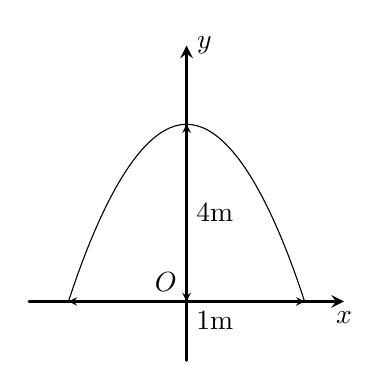
\begin{tikzpicture}[scale=1, line join=round, line cap=round,>=stealth]
	\draw[->,line width = 1pt] (-2,-2.25)--(-2,-2.25)--(2,-2.25) node[below]{$x$};
	\draw[->,line width = 1pt] (0,-3) --(0,1) node[right]{$y$};
	\draw [<->] (1.5,-2.25)--(-1.5,-2.25);
	\draw [<->] (0,0)--(0,-2.25);
	\draw (0,-1.125) node[right]{$4 \mathrm{m}$};
	\draw (0,-2.25) node[below right]{$1 \mathrm{m}$} ;
	\draw (0,-2.25) node[above left]{$O$} ;
	\draw (0,0) parabola (1.5,-2.25) ;
	\draw (0,0) parabola (-1.5,-2.25) ;
	\end{tikzpicture}	
	}
	\noindent Thể tích phần không gian lối đi giới hạn giữa hai cửa là $ 8\cdot \dfrac{8}{3}=\dfrac{64}{3}\approx 21{,}3$ m$^3$.
	}
\end{ex}
\begin{ex}%[2D4V3-1]
	\immini{Trong mặt phẳng tọa độ $Oxy$, cho hình chữ nhật $(H)$ có một cạnh nằm trên trục hoành và có hai đỉnh trên một đường chéo là $A(-1;0)$ và $C\left( a;\sqrt{a}\right)$, với $a>0$. Biết rằng đồ thị của hàm số $y=\sqrt{x}$ chia hình $(H)$ thành hai phần có diện tích bằng nhau. Tìm $a$.	\shortans{$3$}
	}{\begin{tikzpicture}[line join=round, line cap=round,>=stealth,scale=1]
	\tikzset{label style/.style={font=\footnotesize}}
	\draw[->] (-1.6,0)--(4,0) node[below left] {$x$};
	\draw[->] (0,-0.4)--(0,2.5) node[below left] {$y$};
	\draw (0,0) node [below left] {$O$};
	\foreach \x in {-1,1,2,3}
	\draw[thin] (\x,1pt)--(\x,-1pt) node [below] {$\x$};
	\foreach \y in {1,2}
	\draw[thin] (1pt,\y)--(-1pt,\y) node [below left] {$\y$};
	\draw[samples=200,domain=0:3.5,smooth,variable=\x] plot (\x,{sqrt(\x)});
	\path 
	(-1,0) coordinate (A)
	(-1,1.73) coordinate (D)
	(3,0) coordinate (B)
	(3,1.73) coordinate (C)
	;
	\foreach \p/\q in {A/135,B/45,C/80,D/135}
	\fill[black] (\p) circle (1.0pt) ($(\p)+(\q:3mm)$) node{$\p$};
	\draw[pattern = north east lines, line width = 1.2pt,draw=none] (0,0)%
	plot[domain=0:3] (\x,{sqrt(\x)})--(3,1.73) -- (3,0)--cycle;
	\draw (A)--(D)--(C)--(B);
	\end{tikzpicture}}
	\loigiai{
	\begin{center}
	\begin{tikzpicture}[line join=round, line cap=round,>=stealth,scale=1.5]
	\tikzset{label style/.style={font=\footnotesize}}
	\draw[->] (-1.6,0)--(4,0) node[below left] {$x$};
	\draw[->] (0,-0.4)--(0,2.5) node[below left] {$y$};
	\draw (0,0) node [below left] {$O$};
	\foreach \x in {-1,1,2,3}
	\draw[thin] (\x,1pt)--(\x,-1pt) node [below] {$\x$};
	\foreach \y in {1,2}
	\draw[thin] (1pt,\y)--(-1pt,\y) node [below left] {$\y$};
	\draw[samples=200,domain=0:3.5,smooth,variable=\x] plot (\x,{sqrt(\x)});
	\path 
	(-1,0) coordinate (A)
	(-1,1.73) coordinate (D)
	(3,0) coordinate (B)
	(3,1.73) coordinate (C)
	;
	\foreach \p/\q in {A/135,B/45,C/80,D/135}
	\fill[black] (\p) circle (1.0pt) ($(\p)+(\q:3mm)$) node{$\p$};
	\draw[pattern = north east lines, line width = 1.2pt,draw=none] (0,0)%
	plot[domain=0:3] (\x,{sqrt(\x)})--(3,1.73) -- (3,0)--cycle;
	\draw (A)--(D)--(C)--(B);
	\end{tikzpicture}
	\end{center}
	Gọi $ABCD$ là hình chữ nhật $(H)$ với $AB$ nằm trên trục $Ox$.\\
	Nhận thấy đồ thị hàm số $y=\sqrt{x}$ cắt trục hoành tại điểm có hoành độ bằng $0$ và đi qua $C(a;\sqrt{a}).$\\
	Do đó nó chia hình chữ nhật $ABCD$ ra làm 2 phần có diện tích lần lượt là $S_1$, $S_2$.\\
	Gọi $S_1$ là phần diện tích hình phẳng giới hạn bởi các đường $y=\sqrt{x}$, trục $Ox$, $x=0$, $x=a$ và $S_2$ là phần diện tích còn lại.\\
	Ta có $S_1=\displaystyle\int\limits_{0}^{a} \sqrt{x} \mathrm{\,d}x$.\\
	Đặt $t=\sqrt{x}\Rightarrow t^2=x\Rightarrow 2t\mathrm{\,d}t =\mathrm{\,d}x$.\\
	Khi $x=0\Rightarrow t=0$, $x=a\Rightarrow t=\sqrt{a}$.\\
	Do đó $S_1=\displaystyle\int\limits_{0}^{\sqrt{a}} 2t^2 \mathrm{\,d}t =\left(\dfrac{2}{3}t^3\right)\bigg |_0^{\sqrt{a}}=\dfrac{2a\sqrt{a}}{3}$.\\
	Hình chữ nhật $ABCD$ có $AB=a+1$, $AD=\sqrt{a}$.\\
	Khi đó $S_2=S_{ABCD}-S_1=\sqrt{a}(a+1)-\dfrac{2a\sqrt{a}}{3}=\dfrac{a\sqrt{a}}{3}+\sqrt{a}$.\\
	Theo đề bài ta có $S_1=S_2\Leftrightarrow \dfrac{2a\sqrt{a}}{3}=\dfrac{a\sqrt{a}}{3}+\sqrt{a}\Leftrightarrow a\sqrt{a}=3\sqrt{a}\Leftrightarrow a=3$ (do $a>0$).
	}
\end{ex}
\begin{ex}%[2D4C3-1]
	\immini{Cho parabol $(P_1)\colon y = -x^2 + 4$ cắt trục hoành tại hai điểm $A, B$ và đường thẳng $d\colon y = a\left( 0 < a < 4\right)$. Xét parabol $(P_2)$ đi qua $A, B$ và có đỉnh thuộc đường thẳng $y = a$. Gọi $S_1$ là diện tích hình phẳng giới hạn bởi $(P_1)$ và $d$, $S_2$ là diện tích hình phẳng giới hạn bởi $(P_2)$ và trục hoành. Biết $S_1 = S_2$ (tham khảo hình vẽ bên). Tính $T = a^3 - 8a^2 + 48a$.
	\shortans{$64$}
	}
	{\begin{tikzpicture}[scale=0.7, font=\footnotesize, line join=round, line join=round, line cap = round,>=stealth]
	\draw[->] (-3,0)--(0,0) node[below right]{$O$}--(3,0) node[below]{$x$};
	\draw[->] (0,-1) --(0,5) node[right]{$y$};
	\foreach \x in {}{
	\draw (\x,0) node[below]{$\x$} circle (1pt);}
	\foreach \y in {}{
	\draw (0,\y) node[left]{$\y$} circle (1pt);}
	\draw [domain=-2.1:2.1, samples=100] %
	plot (\x, {-(\x)^2+4});
	\draw [domain=-3:3, samples=100] %
	plot (\x, {1.6}) node[ above]{$y=a$};
	\draw [domain=-2.3:2.3, samples=100] %
	plot (\x, {-0.4*(\x)^2+1.6});
	\path 
	(-2,0) coordinate (A)
	(2,0) coordinate (B)
	;
	\foreach \p/\q in {A/135,B/45}
	\fill[black] (\p) circle (1.0pt) ($(\p)+(\q:3mm)$) node{$\p$};	
	\draw [pattern = north west lines, domain=-1.55:1.55, samples=100] plot (\x, {-(\x)^2+4});
	\draw [pattern = north west lines, domain=-2:2, samples=100] plot (\x, {-0.4*(\x)^2+1.6});
	\end{tikzpicture}}
	\loigiai{Phương trình hoành độ giao điểm của $(P_1)$ và $d\colon y=a$ với $ 0<a<4$ là 
	$$-x^2+4=a\Leftrightarrow \hoac{&x=-\sqrt{4-a}\\ &x=\sqrt{4-a}}.$$
	Ta có $S_1 = \displaystyle\int\limits_{-\sqrt{4-a}}^{\sqrt{4-a}} \left( -x^2 + 4 - a\right)\mathrm{\,d}x =\left. \left( -\dfrac{1}{3}x^3 + \left( 4-a\right)x\right)\right|_{-\sqrt{4-a}}^{\sqrt{4-a}} = \dfrac{4}{3}\left( 4-a\right) \sqrt{4-a}$.\\
	$S_2 = \displaystyle\int\limits_{-2}^2 \left( -\dfrac{a}{4}x^2 + a\right)\mathrm{\,d}x =\left. \left( -\dfrac{a}{12}x^3 + ax\right) \right|_{-2}^2 = \dfrac{8a}{3}$.\\
	Mà $S_1 = S_2 \Leftrightarrow \left( 4 - a\right)\sqrt{4 - a} = 2a \Leftrightarrow a^3- 8a^2 + 48a = 64$.
	}
\end{ex}
\begin{ex}%[2D4C3-2]
	\immini{Một hoa văn trang trí được tạo ra từ một miếng bìa hình vuông cạnh bằng $10$ cm bằng cách khoét đi bốn phần bằng nhau có hình dạng parabol như hình vẽ bên. Biết $ AB=5$ cm, $OH=4$ cm. Tính diện tích của bề mặt hoa văn đó (đơn vị: cm$^2$) (kết quả làm tròn đến chữ số thập phân thứ nhất).
	\shortans{$46{,}7$}
	}{\begin{tikzpicture}[scale=0.9, font=\footnotesize, line join=round, line cap=round,>=stealth]
	\tikzset{label style/.style={font=\footnotesize}}
	\def \r{0.5*sqrt(3)};
	\coordinate (A) at ($(2,{\r})$);
	\coordinate (B) at ($(2,{-\r})$);
	\coordinate (H) at ($(A)!0.5!(B)$);
	\clip(-2,-2) rectangle (2.5,2);
	\fill [black] (-2,-2) rectangle (2,2);
	\foreach \i in {0,90,180,270}
	\draw [rotate=\i, fill=white,smooth, samples=200] plot [domain={-\r-0.01}:{\r+0.01}] (\x, {2*(\x)^2+0.5});
	\draw (A) node[right]{$ A $}--(B)node[right]{$ B $};
	\draw (0.5, 0) node[left]{$\color{white} O $}--(H)node[right]{$H$};
	\end{tikzpicture}}
	\loigiai{
	Diện tích bề mặt hoa văn là $ S=10^2-4S_0 $, trong đó $ S_0 $ là diện tích của Parabol.
	\immini{Chọn hệ trục tọa độ như hình vẽ bên.\\
	Parabol có đỉnh $ O(0; 0) $ và đi qua điểm $ B\left(\dfrac{5}{2}; 4\right) $ nên có phương trình là $ y=\dfrac{16}{25}x^2 $.\\
	Tính $S_0$. Ta có $S_0=4\cdot 5-2\cdot \displaystyle\int\limits_{0}^{\tfrac{5}{2}}\dfrac{16}{25}x^2\mathrm{\, d}x=\dfrac{40}{3}$ (cm$^2$).\\
	Vậy diện tích bề mặt hoa văn là $ S=100-4\cdot\dfrac{40}{3}=\dfrac{140}{3}\approx 46{,}7$ (cm$^2$).
	}{
	\begin{tikzpicture}[scale=0.7, font=\footnotesize, line join=round, line cap=round,>=stealth]
	\def \xmin{-3.1}
	\def \xmax{3.1}
	\def \ymin{-1.9}
	\def \ymax{5.3}
	\draw[->] (\xmin, 0.) -- (\xmax,0.) node[anchor=north] {$x$};
	\draw[->] (0.,\ymin) -- (0.,\ymax) node[anchor=west] {$y$};
	\clip(\xmin,\ymin) rectangle (\xmax,\ymax);
	\draw[smooth,samples=100,domain=\xmin:\xmax] plot(\x,{0.64*(\x)^2});
	\draw[pattern=north west lines,smooth,samples=100,domain=-2.5:2.5] plot(\x,{0.64*(\x)^2});
	\draw[dashed] (-2.5,0) node[below] {$-\dfrac{5}{2}$} -- (-2.5,4)node[left]{$ A $}--(0,4)node[above left] {$4$}--(2.5,4)node[right]{$ B $}--(2.5,0)node[below]{$ \dfrac{5}{2} $};
	\draw(0,4)node[above right]{$ H $};
	\draw[fill=black] (0,0) circle (1.5pt) node[below left] {$O$};
	\end{tikzpicture}}
	}
\end{ex}
\Closesolutionfile{ans}